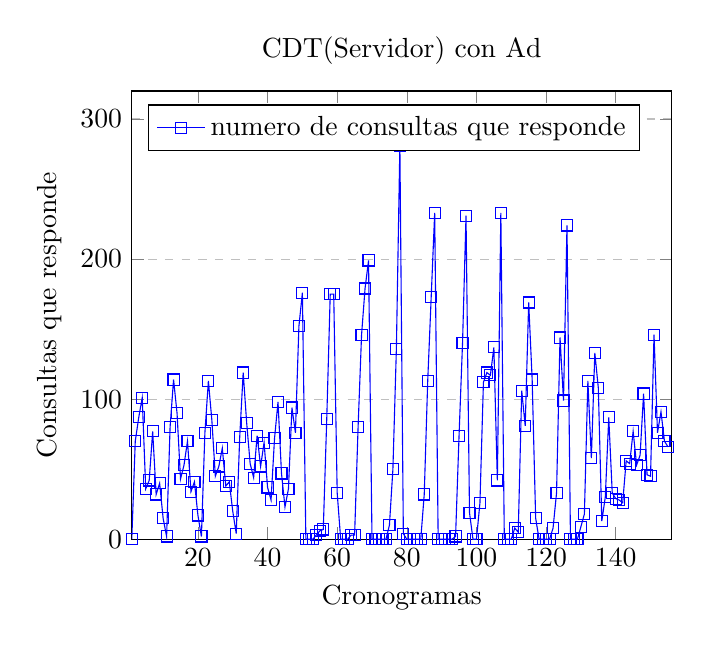
\begin{tikzpicture}
\begin{axis}[
    %CDT = carga de trabajo
    %AEPxT = Algoritmo DETRMINISTA
    title={CDT(Servidor) con Ad},
    xlabel={Cronogramas},
    ylabel={Consultas que responde},
    xmin=1, xmax=156,
    ymin=0, ymax=320,
    xtick={},
    ytick={},
    legend pos=north west,
    ymajorgrids=true,
    grid style=dashed,
]

\addplot[
    color=blue,
    mark=square,
    ]
    coordinates {
   %CARGA DE TRABAJO Servidor
(1,0)
(2,70)
(3,87)
(4,101)
(5,36)
(6,42)
(7,77)
(8,32)
(9,40)
(10,15)
(11,2)
(12,80)
(13,114)
(14,90)
(15,43)
(16,53)
(17,70)
(18,34)
(19,41)
(20,17)
(21,2)
(22,76)
(23,113)
(24,85)
(25,45)
(26,52)
(27,65)
(28,38)
(29,41)
(30,20)
(31,4)
(32,73)
(33,119)
(34,83)
(35,54)
(36,44)
(37,74)
(38,52)
(39,69)
(40,37)
(41,28)
(42,72)
(43,98)
(44,47)
(45,23)
(46,36)
(47,94)
(48,76)
(49,152)
(50,176)
(51,0)
(52,0)
(53,0)
(54,3)
(55,6)
(56,7)
(57,86)
(58,175)
(59,175)
(60,33)
(61,0)
(62,0)
(63,0)
(64,3)
(65,3)
(66,80)
(67,146)
(68,179)
(69,199)
(70,0)
(71,0)
(72,0)
(73,0)
(74,0)
(75,10)
(76,50)
(77,136)
(78,281)
(79,4)
(80,0)
(81,0)
(82,0)
(83,0)
(84,0)
(85,32)
(86,113)
(87,173)
(88,233)
(89,0)
(90,0)
(91,0)
(92,0)
(93,0)
(94,2)
(95,74)
(96,140)
(97,231)
(98,19)
(99,0)
(100,0)
(101,26)
(102,112)
(103,119)
(104,117)
(105,137)
(106,42)
(107,233)
(108,0)
(109,0)
(110,0)
(111,8)
(112,5)
(113,106)
(114,81)
(115,169)
(116,114)
(117,15)
(118,0)
(119,0)
(120,0)
(121,0)
(122,8)
(123,33)
(124,144)
(125,99)
(126,224)
(127,0)
(128,0)
(129,0)
(130,9)
(131,18)
(132,113)
(133,58)
(134,133)
(135,108)
(136,13)
(137,30)
(138,87)
(139,33)
(140,29)
(141,28)
(142,26)
(143,56)
(144,54)
(145,77)
(146,53)
(147,60)
(148,104)
(149,46)
(150,45)
(151,146)
(152,76)
(153,91)
(154,70)
(155,66)
    };
    \legend{numero de consultas que responde}

\end{axis}
\end{tikzpicture}
